\documentclass{bfh}
\usepackage[numbers]{natbib}
\usepackage[nohyperlinks]{acronym}

\title{Bachelor Thesis}
\subtitle{An Android Client for Bitmessage}
\author{Christian Basler}
\advisor{Kai Brünnler}
\expert{Daniel Voisard}
\date{\today}

\newcommand{\abbr}[1]{\textbf{#1}}

\begin{document}
  \maketitle

  \tableofcontents

  \newpage
  \section*{Abstract}

  Even if we use encryption, we reveal a lot about ourselves in the metadata we produce. Bitmessage prevents this by distributing a message in a way that it's not possible to find out which was the intended recipient.
  
  This thesis aims to develop an Android client for the Bitmessage protocol.
  
  \section*{Abbreviations}
  \begin{acronym}[Bash]
    \acro{POW}    {Proof of Work}
    \acro{PGP}    {Pretty Goot Privacy}
    \acro{MIME}   {Multipurpose Internet Mail Extensions}
    \acro{S/MIME} {Secure/\acs{MIME}}
    \acro{CPU}    {Central Processing Unit}
    \acro{JDBC}   {Java Database Connectivity}
    \acro{API}    {Application Programming Interface}
    \acro{DOS}    {Denial of Service}
  \end{acronym}

  \newpage

  \section{Introduction}

  \subsection{What is Metadata?}

  Metadata is information about data we create or access. This could be the websites we visit, what tv programmes we watch, or the sender, recipient, time, which mail client was used, maybe even where it was sent from and what anti-virus is used. The volume and quality of metadata greatly depends on the kind of data and the software used to create it.

  While encryption technology like \ac{PGP} or \acs{S/MIME} provides a secure way to protect content from prying eyes, it can't hide the header information: sender, recipient, subject and possibly much more.

  Ever since the revelations of whistleblower Edward Snowden we learned that metadata --- most notably information about who communicates with whom --- is equally interesting and much easier to analyse than the actual content.\cite{guardian:metadata}

  \subsection{How Can We Hide Metadata?}

  With e-mail, all metadata is plain text, even for encrypted messages. We might be able to encrypt the connection to the e-mail provider, and they might or might not encrypt their connections to other providers. We can only hope that both our and the recipient's e-mail provider are both trustworthy and competent. Can we really expect that from something we get for free? And can we be sure they're not forced to release what they know to some agency?\cite{yale:nsl}

  With Bitmessage we send a message to a sufficiently large number of participants, with the intended recipient among them. Content is encrypted such that only the person in possession of the private key can decrypt it. All participants try to do this in order to find their messages.

  \subsection{What is Bitmessage}
  
  Bitmessage is a peer to peer protocol building a mesh network among the participating clients. Every client tries to maintain multiple connections to other network nodes and has a full copy of every current object.
  
  Objects are encrypted using a public key. Every client tries to decrypt each object using its private keys, processing the ones where it succeeds.
  
  A big advantage of Bitmessage is its inherent key management. The address contains a hash of the public key, and retrieving said key is an integral part of the protocol.


  \subsubsection{Bitmessage Commands}

  Commands are messages between nodes, used to initialize a connection and exchange information about the network and available objects.

  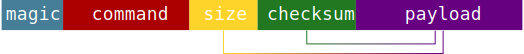
\includegraphics[width=\textwidth]{images/command.pdf}

  The \textbf{magic} is a number to mark the beginning of a command. It is set to \texttt{0xE9BEB4D9}, but \textit{could} be changed for test clients so they don't inadvertently connect to the real network.

  A \textbf{command} defines how the payload looks like and what the node is supposed to do with it. The commands used by the Bitmessage protocol are \textit{version}, \textit{verack}, \textit{addr}, \textit{inv}, \textit{getdata} and \textit{object}. Their uses are specified in the Bitmessage Protocol Specification.\cite{wiki:protocol}

  \textbf{Size} defines how many bytes of payload need to be read.

  The \textbf{checksum} is used to prevent transmission errors.

  \textbf{Payload} is the data that belongs to a command. It could be anything from empty to an object containing a message.


  \subsubsection{Bitmessage Objects}
  Objects are distributed throughout the network using the "object" command. With exception of some legacy objects, they are signed and encrypted.

  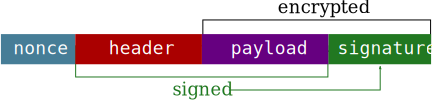
\includegraphics[width=\textwidth]{images/object.pdf}

  To prevent malicious flooding of the network and, to a lesser extent, spam, a \textbf{nonce} needs to be found such that a specific hash over the whole object represents a number lower than a calculated threshold. This is called \ac{POW}.

  The object \textbf{header} consists of the expiration time, object type and version, stream number and the actual payload. (Streams ar an optimisation feature of the protocol, so it stays somewhat scalable if many people start using Bitmessage.)
  
  The \textbf{payload} contains the actual data, depending on the message type.
  
  The \textbf{signature} covers everything except the nonce and is encrypted along with the payload, thus covering the unencrypted payload.

  There are four different types of objects in the Bitmessage protocol: \textit{getpubkey} is used to request a public key to some address, \textit{pubkey} contains said public key, \textit{msg} is a typical person-to-person message, and \textit{broadcast} is a message that is broadcast to anyone who subscribed to the sending address --- which needs to be known in order to subscribe.


  \subsubsection{Encryption}


(TODO)\newpage

  \subsection{Current state -- what is missing?}
  Until recently there was no mobile client for Bitmessage, and the client that turned up since is very wasteful to the devices resources, draining the battery in little time. The alternative is to use an e-mail relay server, but this means to give up the private key to this server and end-to-end encryption is much more difficult to achieve. Therefore this might not be a viable option, especially if you can't run your own server.

  \subsection{How should it be?}
  We need mobile Bitmessage clients that allows the user to choose their levels of convenience, privacy and resource hunger. There will always be trade-offs between needed traffic, battery use and privacy, and for each user the answer might look slightly different.

  \subsection{Why is it hard to do?}
  Bitmessage is very wasteful with resources by design. All messages are being sent to and stored on all nodes, and to protect the network \ac{POW} is required for all objects that are distributed, meaning some very \acs{CPU}-heavy calculations need to be done. The protocol wasn't developed with mobile users in mind, and while smartphones are getting increasingly powerful, there is at least the issue of battery use to watch out for, and many users have limited traffic on their data plan.

  \subsection{Why me, and how do I intend to do it?}
  I have seven years of experience developing Java applications, and was programming Android apps from the moment I had my ``Android Dev Phone 1''. As I developed Jabit, a Java implementation of the Bitmessage client, as my last project, I also have great knowledge about the Bitmessage protocol.

  There are a few optimisations that I intend to do:
  \begin{itemize}
    \item Connect to only one reliable node instead of eight random nodes. This should reduce battery usage, but yields some risk if the node is compromised. Also, the node must forward all messages to all connected mobile clients instead of the default eight random nodes.
    \item Don't save objects we can't decrypt. We can solely save their hashes, but this means we're using the network without supporting it. This also might be an attack vector.
    \item Only connect to the network if we're on Wi-Fi and charging. This means of course that we'll only receive messages when we're connected with a Wi-Fi and charging.
  \end{itemize}
  Of course every option has its own drawbacks, so they will be configurable. As for the \ac{POW}: Jabit highly optimises its calculation, which might be enough for modern smartphones.

  Further optimisations might introduce a server component that \textit{might} do
  \begin{itemize}
    \item \acl{POW}
    \item Request public keys, requiring us to give up some anonymity towards the server.
    \item Inform the client about new messages sent to its addresses. This would mean to give up our anonymity towards the server in the best case (which isn't supported by the protocol yet), towards the whole network (which is somewhat supported), or give up the private key to the server (which, for many users, is unacceptable).
  \end{itemize}

  To find out what is actually necessary, a naive impementation will be done first.

  \subsection{The Jabit Bitmessage Library}
  Jabit war developed as a preparing project for this thesis.

TODO


  \subsubsection{Architecture}
  Jabit follows the Ports and Adapters architecture. There is a domain module which contains all the data types and most parts of the protocol implementation, and provides several ports, to which adapters can be attached. Adapters include the data repositories, network code and, more recently, cryptography (see \ref{subsec:bcvssc} \nameref{subsec:bcvssc}{}).

  \begin{center}
    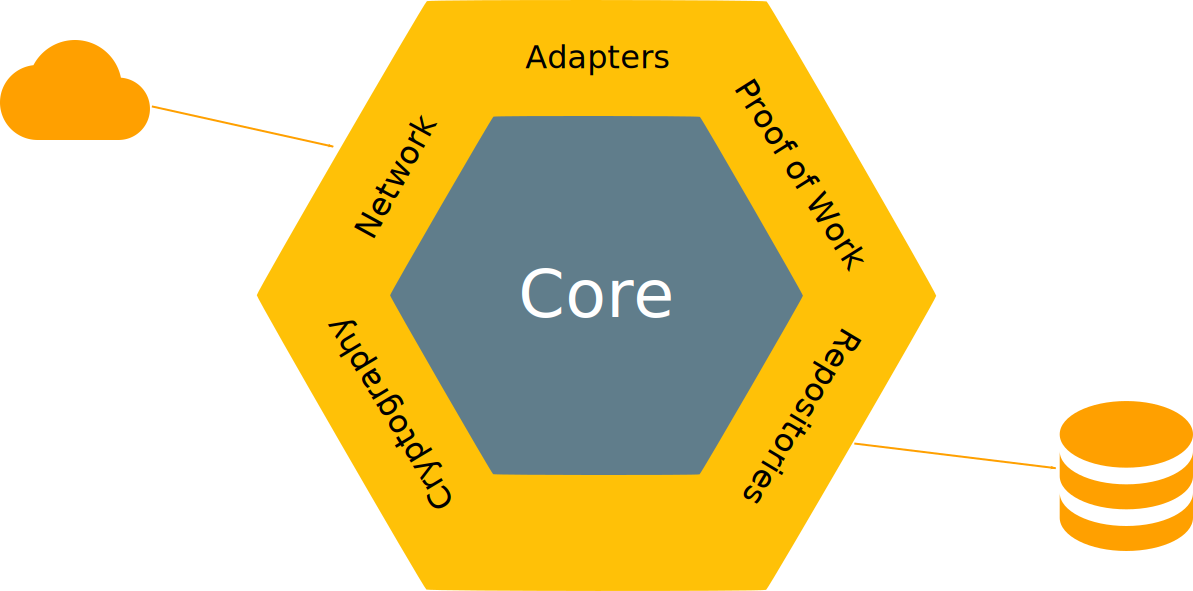
\includegraphics[width=0.5 \textwidth]{images/ports_and_adapters.pdf}
  \end{center}

  \section{Naive Implementation}
  
  The naive implementation attempts to use the Jabit Bitmessage library as it is, with as little mobile optimisations as possible. The plan was to either discard or improve it afterwards. Fortunately improvement was possible.

  \subsection{Unexpected Problems}
  Most problems can be summarised as this: Android builds on the Java language, but not on the Java platform. While the programming language is the same and most libraries can be used without any restrictions, there are some subtle differences that make a programmer's life hard --- some due to the limited resources of a mobile handset, some due to design decicions made by the Android development team.
  
  \subsubsection{Bouncy Castle vs. Spongy Castle}
  \label{subsec:bcvssc}
  Jabit heavily relies on Bouncy Castle, a very popular open source encryption library.\cite{bouncy} Unfortunately, Android ships with a broken version of Bouncy Castle. Even worse, when building an Android app, the toolchain just discards any Bouncy Castle dependencies in favour of the built-in, broken version.

  Some people recognised this problem, and built a fork of Bouncy Castle, called Spongy Castle. It basically just replaces “Bouncy” with “Spongy” wherever necessary, so it doesn’t get discarded during the build process. This works fine and is quite easily done. Unfortunately, this doesn’t work on the Desktop.

  The Oracle JVM requires Security Providers to be signed, which is done for Bouncy Castle builds, but not so for the Spongy derivation. As forking Jabit wasn’t an option, the whole cryptography part had to be refactored into an exchangeable module, and implemented twice, in both a bouncy and a spongy manifestation.

  \subsubsection{JDBC}
  Android has its own API to access the included SQLite database. While it’s a nice, easy to use \ac{API}, the Android team didn’t deem it necessary to support \ac{JDBC}, which is the Java standard API to connect to databases.

  There is an open source project attempting to implement a \ac{JDBC} driver for Android’s SQLite database called SQLDroid,\footnote{\url{https://github.com/SQLDroid/SQLDroid}} which looked very promising. Unfortunately, it lacks essential features, such as returning the automatically generated key of an inserted row. Even worse, it doesn't have the courtesy of throwing a NotImplementedException for missing features, instead it just does nothing and returns null where a result is required, making debugging unnecessarily tedious.

  Unfortunately, discovering SQLDroid was unfit for the job took more time than reimplementing all repositories using the Android database API. As they were already implemented as adapters, no change was necessary on the Jabit library. Many changes were made in the futile attempt to use JDBC though, most of them only to be reverted later on.

  \subsection{Expected Problems}
  Those problems were to be expected and need to be fixed as part of this thesis.

  \subsubsection{\acl{POW}}
  Although modern smartphones tend to have faster processors than cheap personal computers, \ac{POW} for sending a public key takes around 15 minutes on a device with four cores at 2.5 GHz. Even worse, during this time it uses so much power that the device discharges even when connected to a power supply.

  \section{Android Specific Challenges}
  \subsection{Application Lifecycle}
  As with any good mobile system, Android doesn't hesitate to end all threads of an application running in background, in order to save resources. Consequently anything that should be kept alive -- network connections and \ac{POW} come to mind -- needs special treatment. This is done through foreground services. The networking part and \ac{POW} hence needed to be moved into separate services. While not difficult, it needed some research to find out how it should best be done in our case.

  \begin{center}
    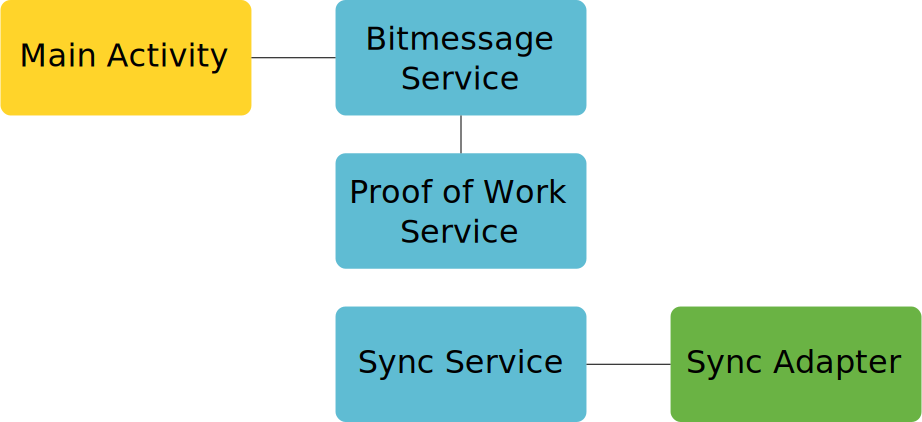
\includegraphics[width=0.6 \textwidth]{images/services.pdf}
  \end{center}

  \section{Optimisations}
  \subsection{Sync Adapters}
  Android provides an API that can vastly reduce battery usage for apps that regularly update data over the internet. The system triggers synchronisation, so it can optimise its sleep modes. Imagine otherwise, 15 apps synchronising every 15 minutes, one after the other. In the worst case scenario the device would need to wake up every minute, synchronize and could barely go back to sleep before the next app wants to synchronize.

  Although it's not intended, synchronisation can be done within the Bitmessage protocol without any modifications. What is needed is a trusted node that's always available and therefore best run on a proper server. On successful connection all new messages are being exchanged, so we just need to connect, wait until new messages were exchanged, and then disconnect.

  As Jabit is a Java library, it was trivial to create a server application using Spring Boot and Jabit. It turned out though that it's necessary to limit the number of connections in a Bitmessage server, therefore connections are now being severed after 12 hours or when a limit of 100 connections is reached.

  \subsection{Server Side \acl{POW}}
  To reduce power consumption and possibly reduce the time to send a message, \ac{POW} can be calculated by the synchronisation server. This feature needs some changes on both server and client, and some custom extensions to the protocol.

  \subsubsection{Initial Idea}
  The server accepts messages without \ac{POW}, which it will compute and fill in, and then relay that message. Of course this would leave the server extremely vulnerable to \ac{DOS} attacks -- an attacker could just send a bunch of messages and the server would be busy the rest of its life.

  Fortunately, Bitmessage has very secure authentication built in: every message is signed by a private key, and can be securely verified by anyone who knows the sender's address. We'll just send a message to the server that contains the actual message as content. All nonce fields are set to zero. Ther server checks if the sender is on a white list and then calculates the nonce and relays the complete message.

  A broadcast message would be best qualified for this task, as the client wouldn't have to be configured with a recipient address. The server is configured with a list of addresses that are allowed to request \ac{POW} and the client just needs to know the server's IP address or host name.

  \subsubsection{Acknowledging Issues}
  Unfortunately this approach has some issues. For one, sending a message would be very different using this method, requiring some major changes on the client side. Moreover, it would be impossible to generate acknowledgements.

  Acknowledgements are sent from the receiving client to notify the writer that the message was received. Think of it as a stamped addressed envelope delivered with a letter. The acknowledgement is part of the encrypted message the server can't read, so it couldn't calculate its \ac{POW}.

  Jabit doesn't support acknowledgements yet, but it would be a pity to prevent it by design.

  \subsubsection{\ac{POW} Protocol}
  Much of the planned design can be reused -- the encryption used by broadcasts, signing the messages -- but we need a wholly separate protocol, with some extra roundtrips to the server. Now the server just receives the parts needed for \ac{POW} calculation: a hash and a target value.

  When the nonce is found, it's saved on the database. The client will regularly poll for it (e.g. during synchronization cycles) until it retrieves the nonce.

  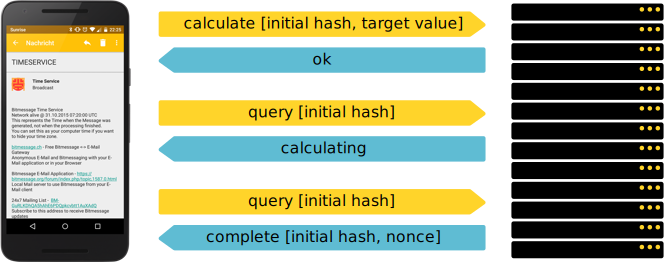
\includegraphics[width=\textwidth]{images/server_pow_protocol.pdf}

  For this feature, a new command was introduced, which needs to be implemented on both server and client. It has the same structure as any Bitmessage command, and \textit{custom} in the command field. As payload it contains a signed and encrypted block, containing the following structure:

TODO: graphical description of the custom POW message

TODO: describe the structure of bitmessage commands in the protocol chapter

  \section{Social and Ethical Consequences}
  

  \newpage
  \bibliographystyle{plain}
  \bibliography{bibliography}

\end{document}